\section{Einrichtung der Eclipse-Arbeitsumgebung}
Für die Einrichtung müssen zunächst grundlegende Vorbereitungen getroffen werden wie beispielsweise die Installation des JavaJDK, Eclipse, Maven sowie einer lokalen PostgreSQL-Datenbank.

Die Installation und Einrichtung wird an dieser Stelle nicht beschrieb. Es wird davon ausgegangen, dass das Vorgehen diesbezüglich bekannt und abrufbereit ist. Sollten bereits ältere Programmversion installiert sein, wird an dieser Stelle empfohlen eine Versionsaktualisierung auf die oben genannten Programmversion durchzuführen.

\subsection{Installation empfohlener Eclipse Plugins}
Wurden alle notwendigen Vorbereitungen getroffen kann mit der Installation des Eclipse-Plugins begonnen werden. Über den Menüpunkt \textsc{Help / Install New Software\ldots} öffnet sich ein Fenster zum hinzufügen neuer Software (z.\,B.\,Plugins).

\subsubsection{jBPM Plugin}
Die benötigte URL, für das in diesem Dokument beschrieben Eclipse-Plugin, lautet: \href{http://downloads.jboss.org/jbpm/release/6.3.0.Final/updatesite/}{http://downloads.jboss.org/jbpm/release/6.3.0.Final/updatesite/}
Diese wird unter \textsc{Work with:} eingetragen und mit einem Klick auf \textsc{Add\ldots} bestätigt. Nach kurzem laden des Inhalts, werden im mittleren Bereich die zur Installation bereitstehenden Pakete angezeigt (siehe Abbildung \ref{fig:install-jbpm-package-list}).\footnote{Farblose Icons weisen auf bereits installierte Plugins hin.}
\begin{figure}[h]
	\centering
	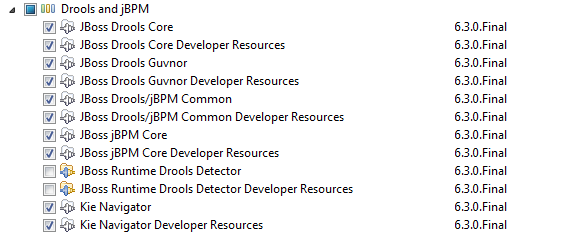
\includegraphics[width=\textwidth]{image/screenshots/install-jbpm-plugin}
	\caption{Liste an jBPM-Paketen für Eclipse-Plugin}\label{fig:install-jbpm-package-list}
\end{figure}

\subsubsection{BPMN2 Modeler Plugin}